% Created 2024-10-24 Thu 20:58
% Intended LaTeX compiler: xelatex

\documentclass[10pt]{beamer}

% fonts
\usepackage{ctex}
\usepackage{fontspec}
\setmainfont{Times New Roman}
\setmonofont{Inconsolata}
\setsansfont{Times New Roman}
\setCJKmainfont{SimSong}
\setCJKsansfont{SimSong}

\usepackage{amsfonts}
\usepackage{amsthm}
\usepackage{bm}
\usepackage{siunitx}
\usepackage{xcolor}

\usepackage{mathrsfs}
% commands
\newcommand{\mr}[1]{\mathrm{#1}}
\newcommand{\mb}[1]{\mathbf{#1}}
\newcommand{\mc}[1]{\mathcal{#1}}
\newcommand{\ms}[1]{\mathscr{#1}}

\usepackage{graphicx}
\usepackage{longtable}
\usepackage{wrapfig}
\usepackage{rotating}
\usepackage[normalem]{ulem}
\usepackage{amsmath}
\usepackage{amssymb}
\usepackage{capt-of}
\usepackage{hyperref}
\usepackage{etoolbox}
\usepackage{pgfopts}
\usepackage{booktabs}
\usepackage[scale=2]{ccicons}
\usetheme[block=fill, progressbar=frametitle]{metropolis}
\useoutertheme{infolines} % 采用 infoline
\useinnertheme{default}
\usecolortheme{custom} % 使用 custom 颜色主题
\setbeamertemplate{blocks}[rounded][shadow=false]
\setbeamertemplate{items}[circle] % circle item symbol
\setbeamertemplate{sections/subsections in toc}[ball] % ball section symbol
\setbeamertemplate{headline}[default] % 不使用 infoline 的 headline
%\setbeamertemplate{footline}[default] % 使用 infoline 的 footline
\setbeamertemplate{frame numbering}[none]
\setbeamertemplate{bibliography item}[text] % 使用 text 的 references 形式
%\setbeamerfont{footnote}{\tiny} % 可选择 tiny footnote
\usetheme{default}
\author{朱宇涛 \quad 报告人:王亚朋}
\date{2024年10月24日}
\title{余波, 能量刻度与 \(\mu\) 寿命测量}
\subtitle{宇宙线粒子探测与物理实验}

\hypersetup{
pdfauthor={朱宇涛 \quad 报告人:王亚朋},
pdftitle={余波, 能量刻度与 \(\mu\) 寿命测量},
pdfkeywords={},
pdfsubject={},
pdfcreator={Emacs 29.1 (Org mode 9.6.6)},
pdflang={Cn},
colorlinks=true,
linkcolor=black
}
\begin{document}

\maketitle
\begin{frame}[label={sec:org55f963c}]{目录}
\tableofcontents
\end{frame}
\section{实验目标}
\label{sec:org09833dd}
\begin{frame}[label={sec:org608b27f}]{实验目标}
\begin{enumerate}
\item 重新测量 \(\mu\) 信号与余波的一些参数;
\item 测量单光子电荷;
\item 进行能量刻度;
\item 测量 \(\mu\) 寿命。
\end{enumerate}
\end{frame}
\section{实验装置}
\label{sec:orgedd1efa}
\begin{frame}[label={sec:org7e65136}]{实验装置}
\begin{figure}[htbp]
\centering
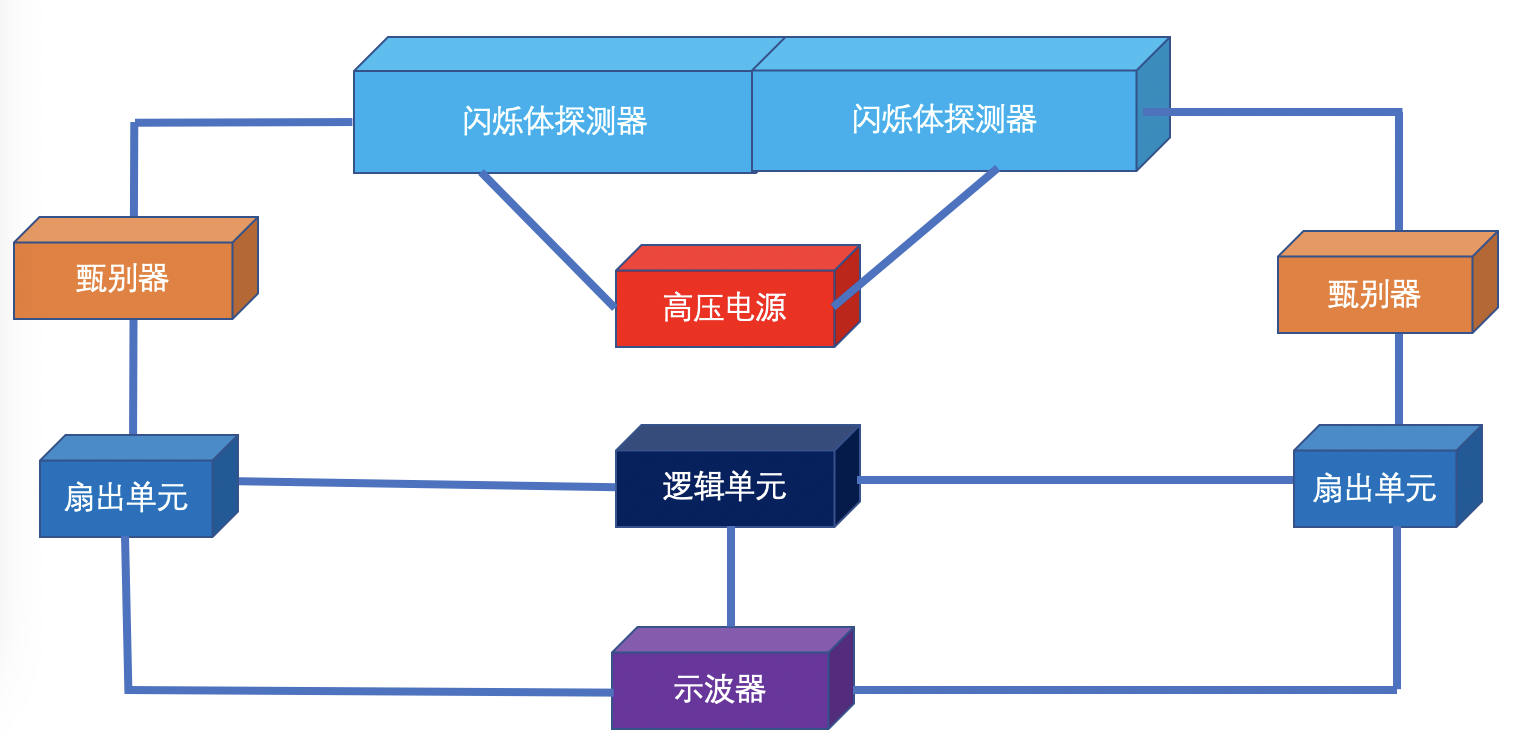
\includegraphics[width=0.8\textwidth]{img/Ex02_20241024164303.png}
\caption{实验装置}
\end{figure}
\end{frame}
\section{实验结果}
\label{sec:org3268965}
\begin{frame}[label={sec:org3ca4ce0}]{\(\mu\) 信号测量}
使用甄别器的 4、7 道(甄别电压 \qty{15}{mV}),测量符合信号。\footnote{后续实验条件不变.}

\begin{itemize}
\item 左:电压 1350V.

信号宽度:\(\Delta X(\mr{CH1}) = \qty{43.4}{ns}\).

计数率:\(n(\mr{CH1}) = \qty{2995}{min^{-1}}\).

\item 右:电压 1500V.

信号宽度:\(\Delta X(\mr{CH2}) = \qty{38.4}{ns}\).

计数率:\(n(\mr{CH2}) = \qty{2014}{min^{-1}}\).

\item 符合

计数率:\(n = \qty{859}{min^{-1}}\).
\end{itemize}

计算得到偶然符合计数率:
\begin{equation}
\label{eq:1}
n_a = \qty{0.176}{min^{-1}}.
\end{equation}
\end{frame}

\begin{frame}[label={sec:org336ccb9}]{\(\mu\) 信号测量}
对闪烁体, 测得长 60.5cm, 宽 15.5cm, 由此可计算 \(\mu\) 通量:

\begin{equation}
\label{eq:2}
\phi_{\mu} = 0.916 \pm \qty{0.031}{min^{-1}cm^{-2}}.
\end{equation}
\end{frame}

\begin{frame}[label={sec:orgd704c4b}]{余波时间分布}
余波出现的概率为 13.9\%.

\begin{columns}
\begin{column}{0.5\columnwidth}
\begin{figure}[htbp]
\centering
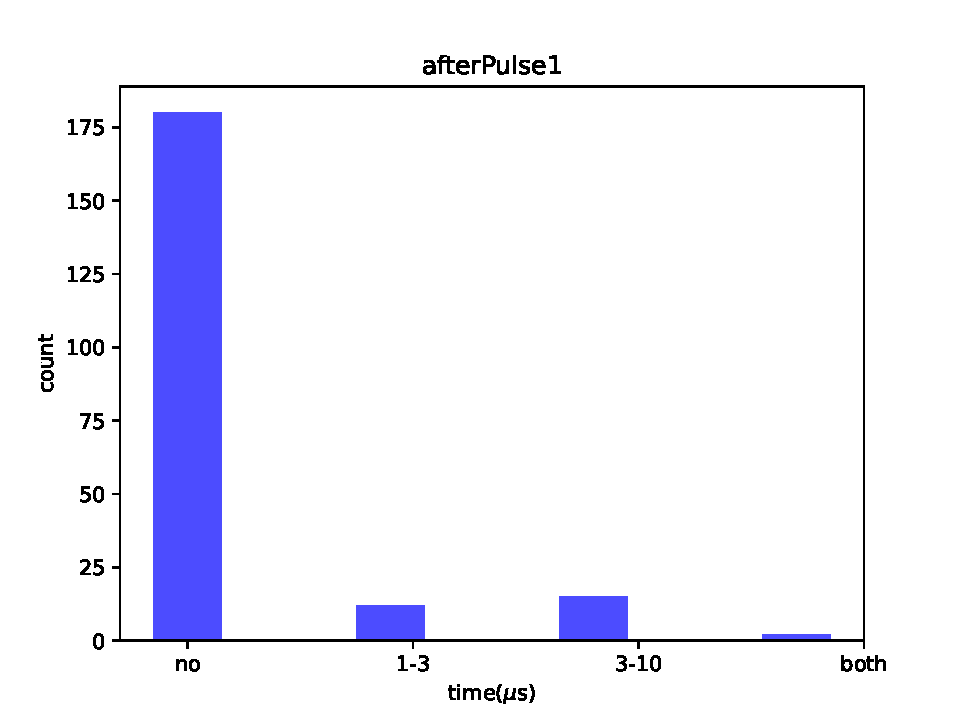
\includegraphics[width=0.9\textwidth]{../../DetectorPerform/afterPulse/fig/afterPulse01.pdf}
\caption{所有信号的余波分布}
\end{figure}
\end{column}

\begin{column}{0.5\columnwidth}
\begin{figure}[htbp]
\centering
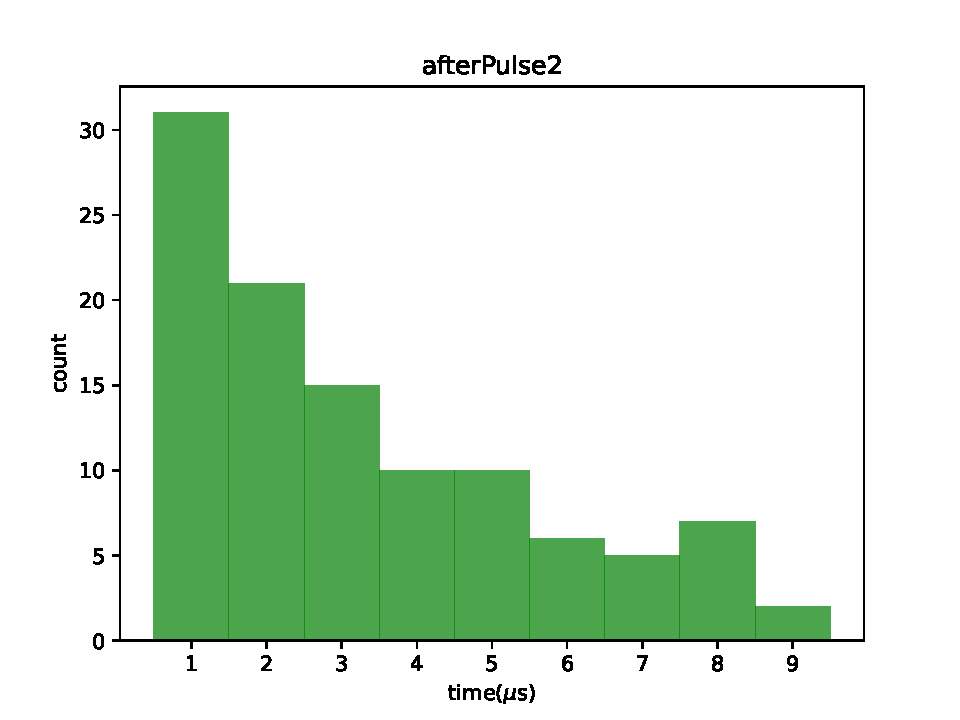
\includegraphics[width=0.9\textwidth]{../../DetectorPerform/afterPulse/fig/afterPulse02.pdf}
\caption{存在余波信号的余波分布}
\end{figure}
\end{column}
\end{columns}
\end{frame}

\begin{frame}[label={sec:org8d0e738}]{余波时间分布}
余波时间分布比较符合指数规律, 对其作拟合得到:

\begin{figure}[htbp]
\centering
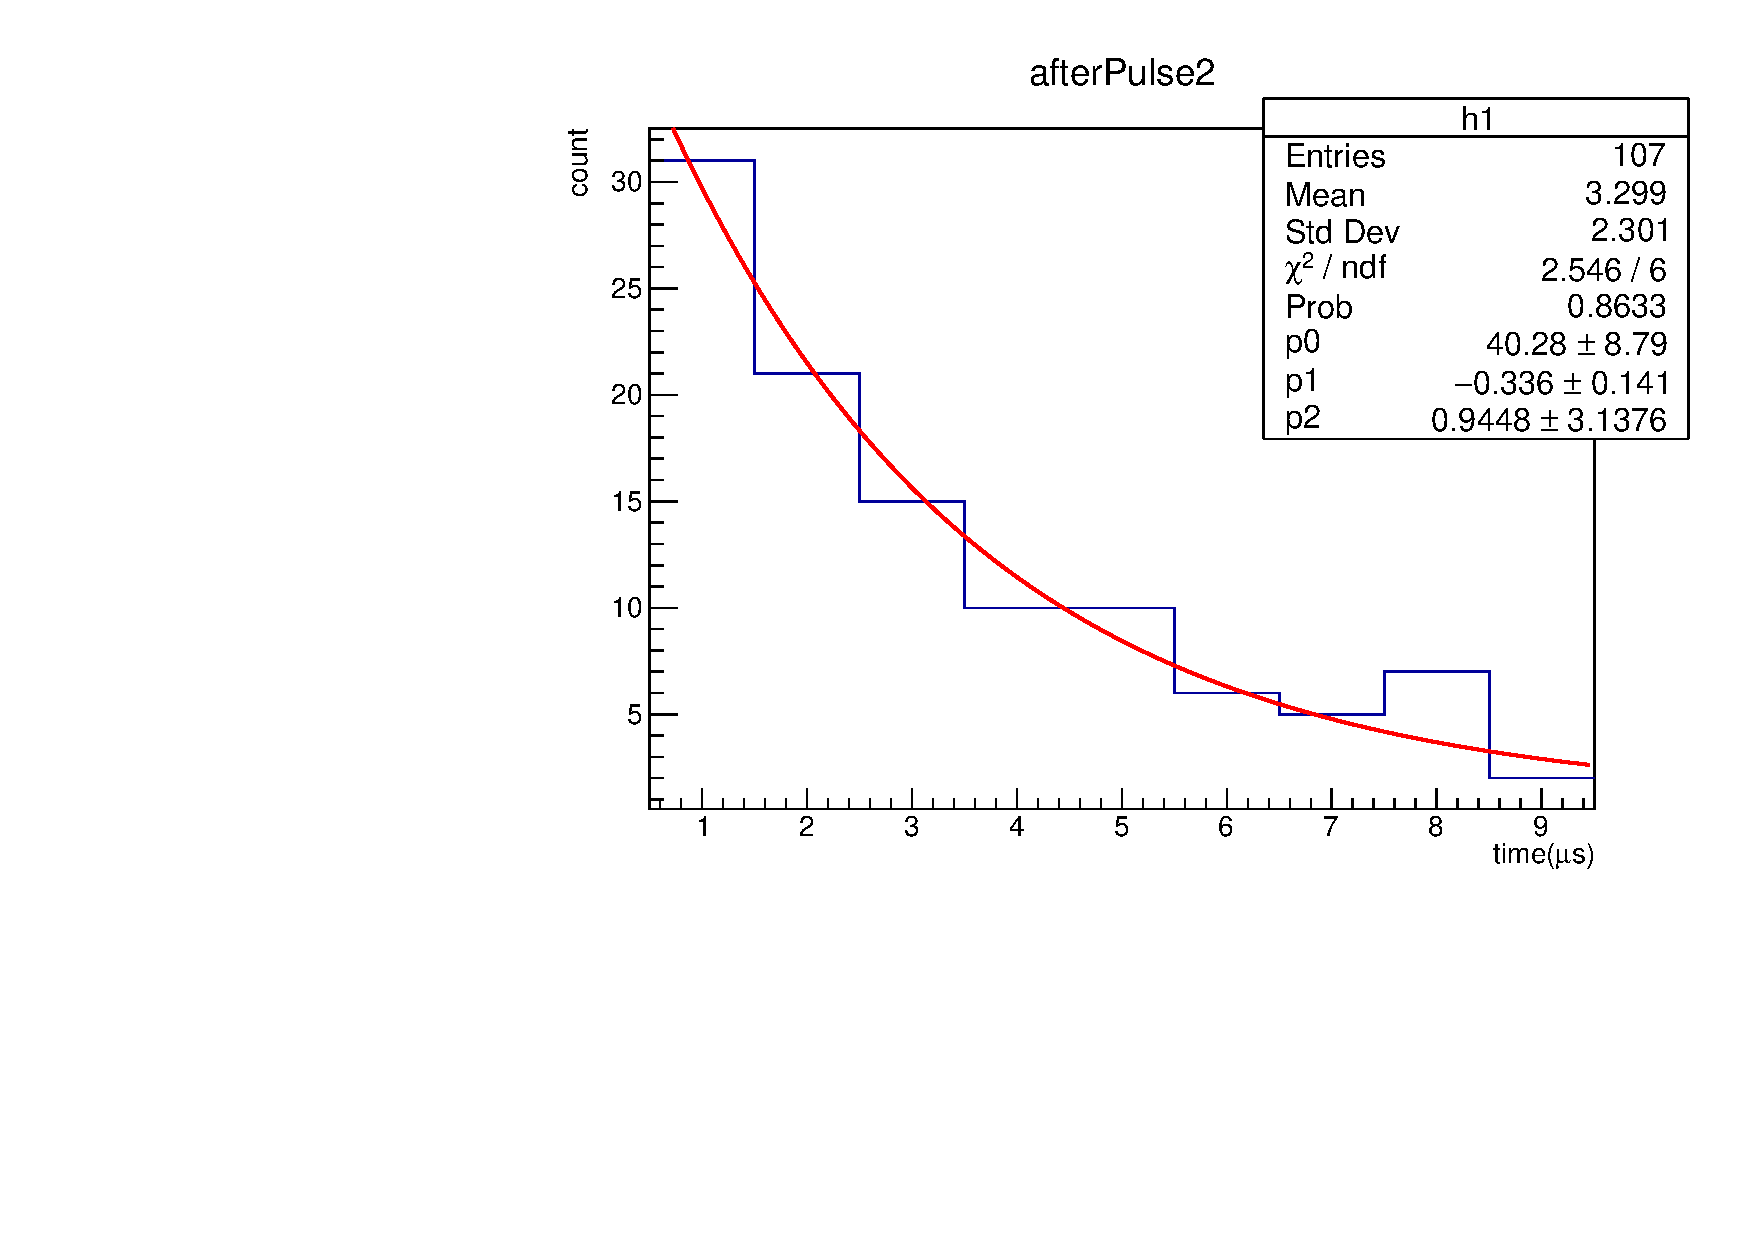
\includegraphics[width=0.6\textwidth]{../../DetectorPerform/afterPulse/fig/afterPulse02r.pdf}
\caption{余波分布拟合}
\end{figure}
\end{frame}

\begin{frame}[label={sec:orgb7cd91f}]{单光子电荷}
\begin{figure}[htbp]
\centering
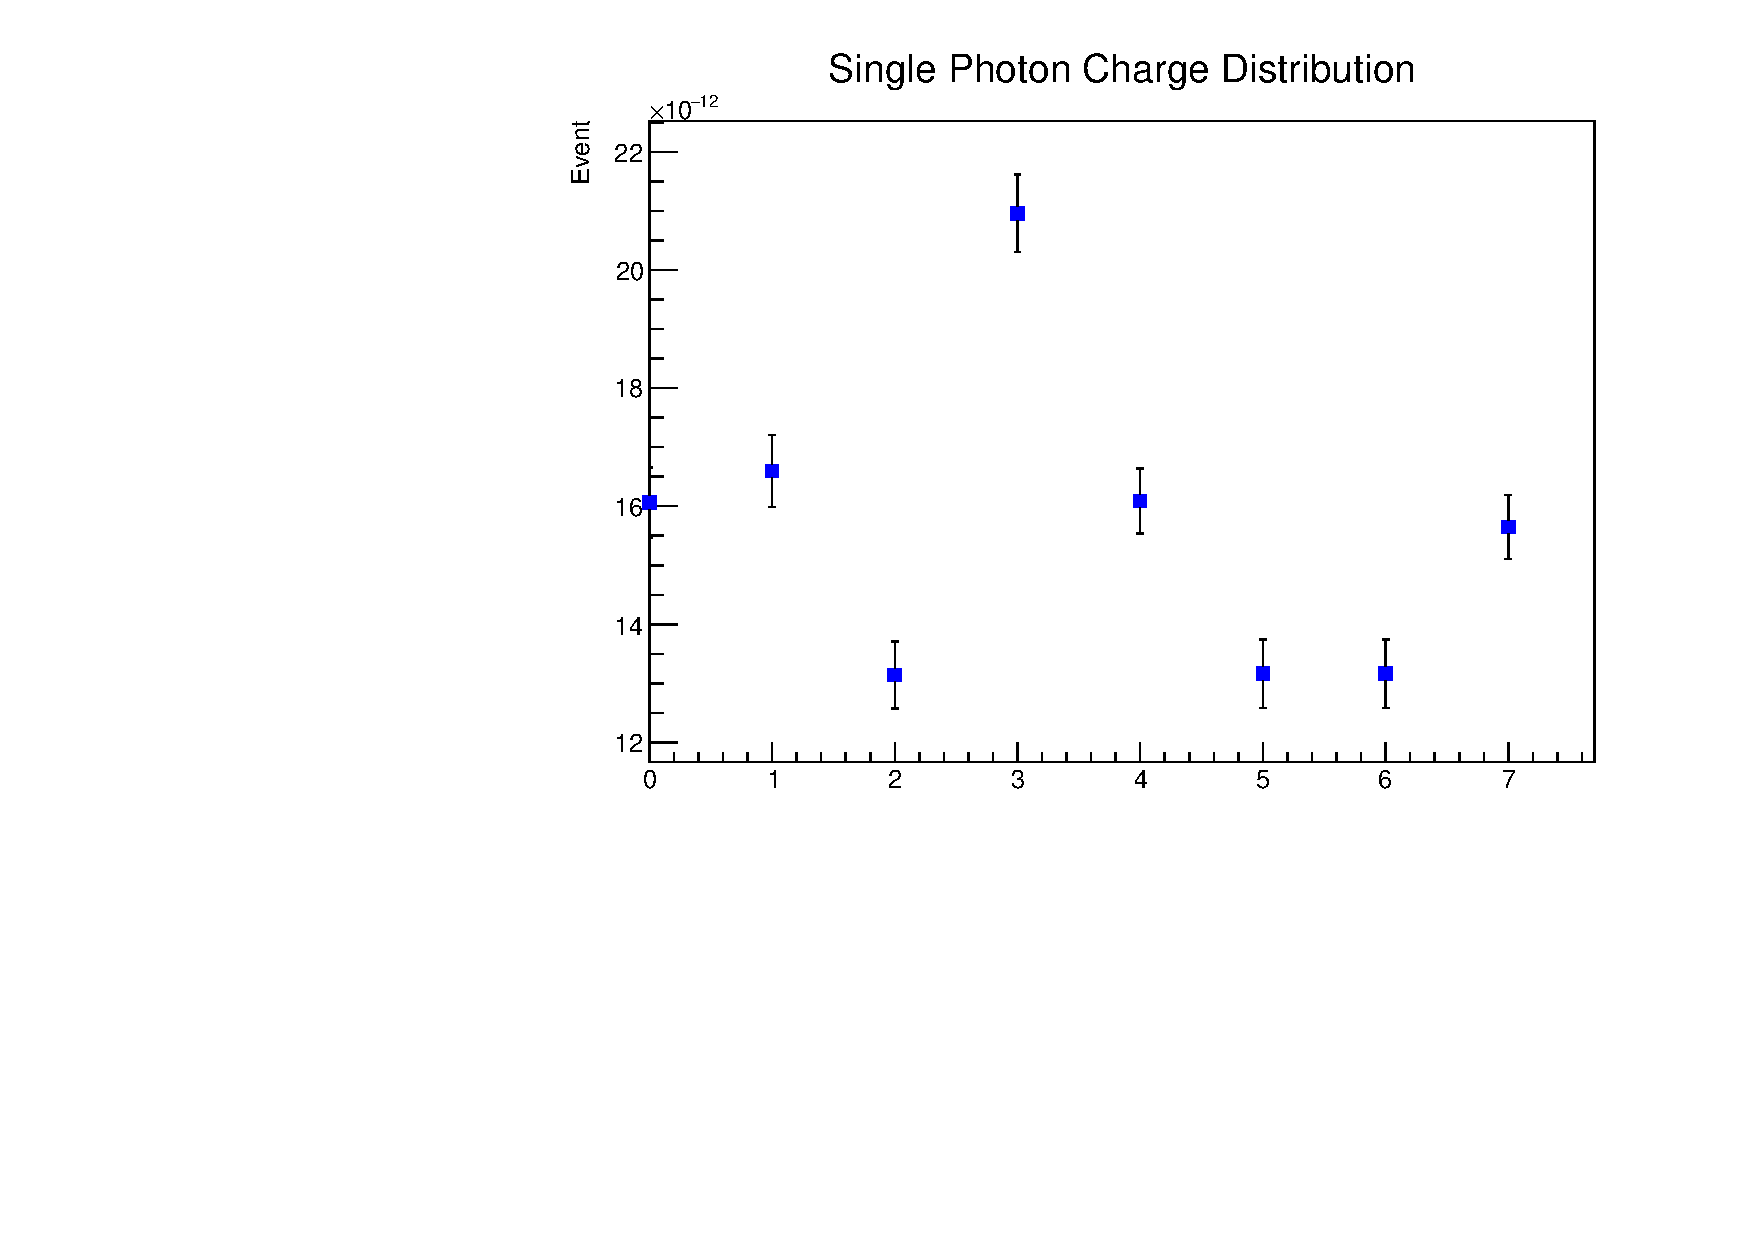
\includegraphics[width=0.6\textwidth]{../../DetectorPerform/SPhoton/SphotonCharge.pdf}
\caption{单光子电荷}
\end{figure}

单光子电荷量:
\begin{equation}
\label{eq:6}
q = (1.560 \pm 0.245)\times\qty{e-11}{V\cdot s}.
\end{equation}
\end{frame}

\begin{frame}[label={sec:orga84c383}]{衰减长度}
考虑 Error Bar, 重新计算衰减长度\footnote{不确定度优于上次结果 (0.1494m).}与相关系数:
\begin{align}
\label{eq:3}
L &= 1.643 \pm \qty{0.131}{m} \\
R^2 &= 0.442.
\end{align}

\begin{columns}
\begin{column}{0.5\columnwidth}
\begin{figure}[htbp]
\centering
\includegraphics[width=0.8\textwidth]{../../DetectorPerform/AttenuationLength/figs/Dist.png}
\caption{衰减长度}
\end{figure}
\end{column}

\begin{column}{0.5\columnwidth}
\begin{figure}[htbp]
\centering
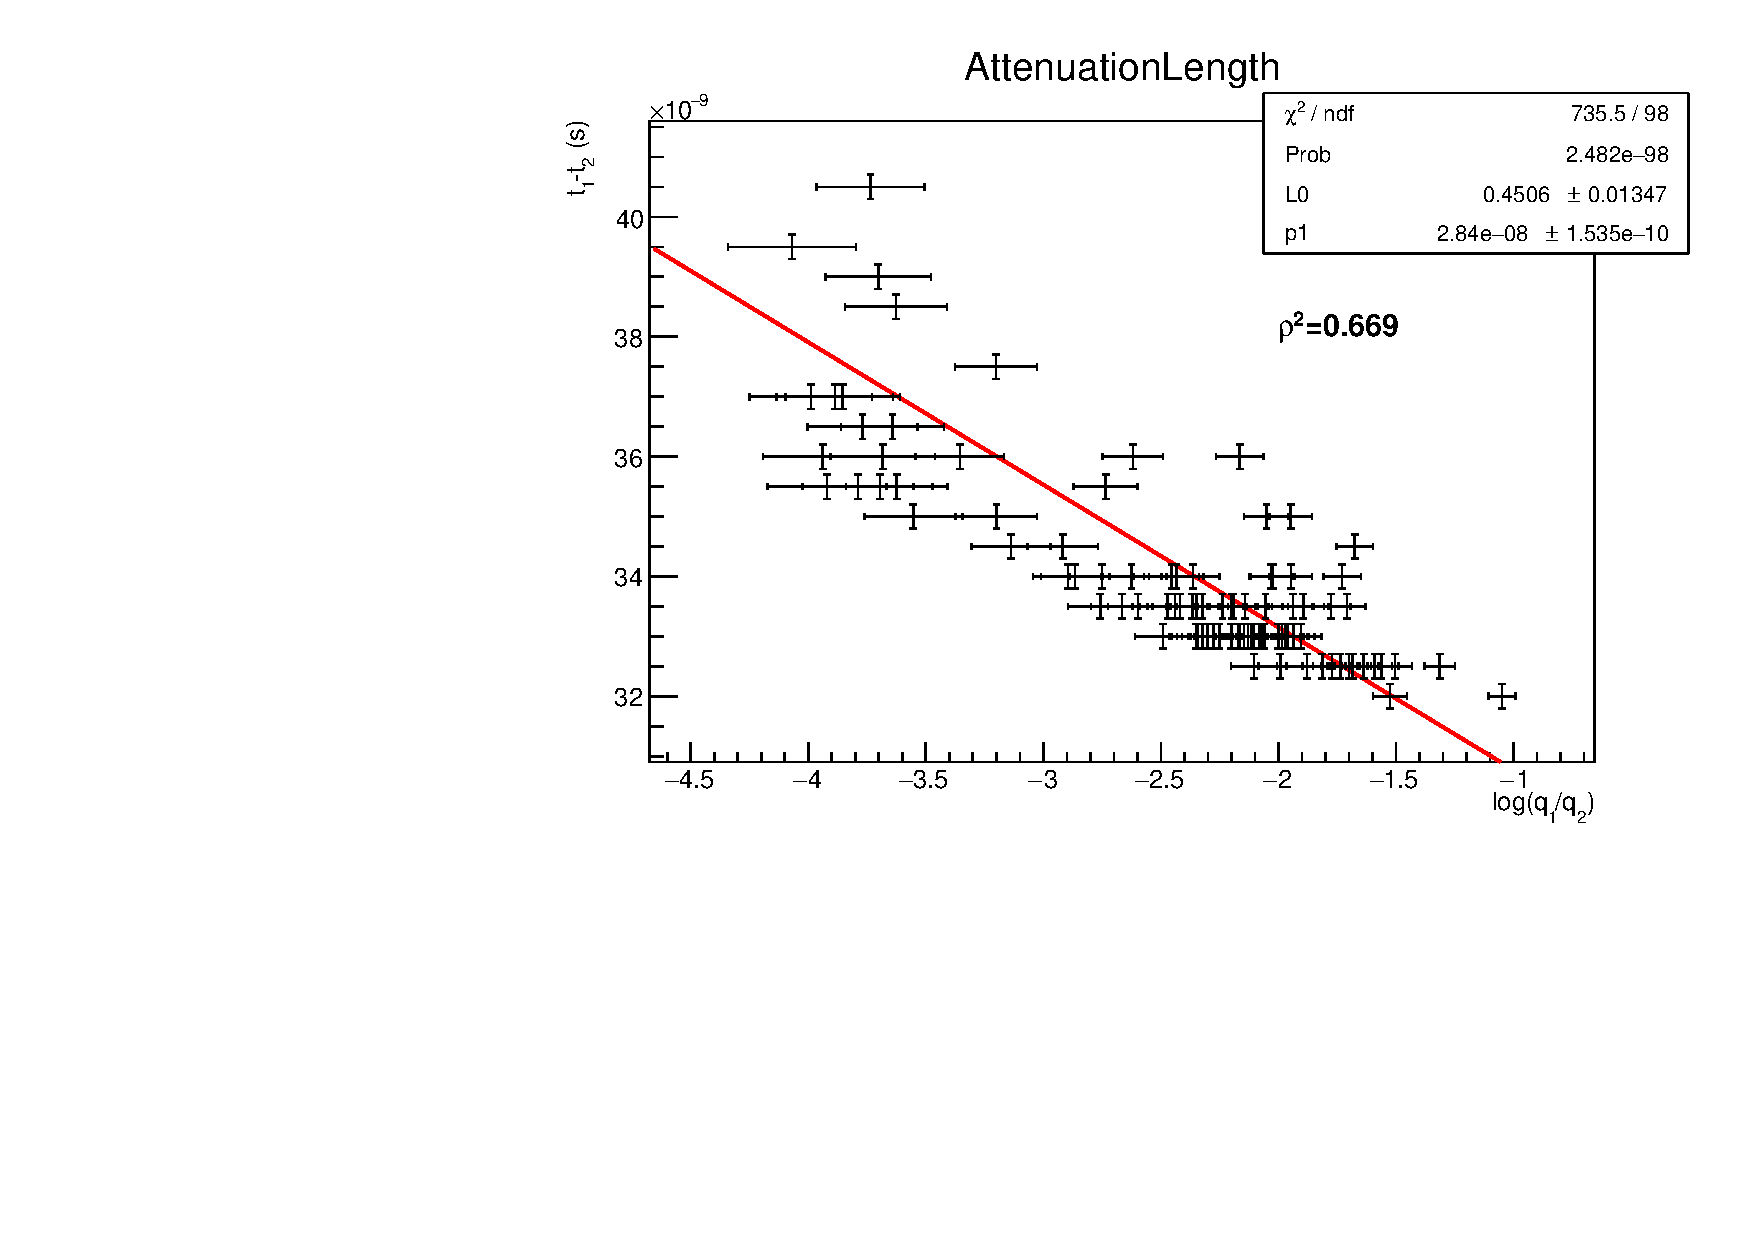
\includegraphics[width=0.8\textwidth]{../../DetectorPerform/AttenuationLength/figs/AttenuationLength.pdf}
\caption{衰减长度 (考虑 Error Bar)}
\end{figure}
\end{column}
\end{columns}
\end{frame}

\begin{frame}[label={sec:org1764341}]{能量刻度}
\begin{figure}[htbp]
\centering
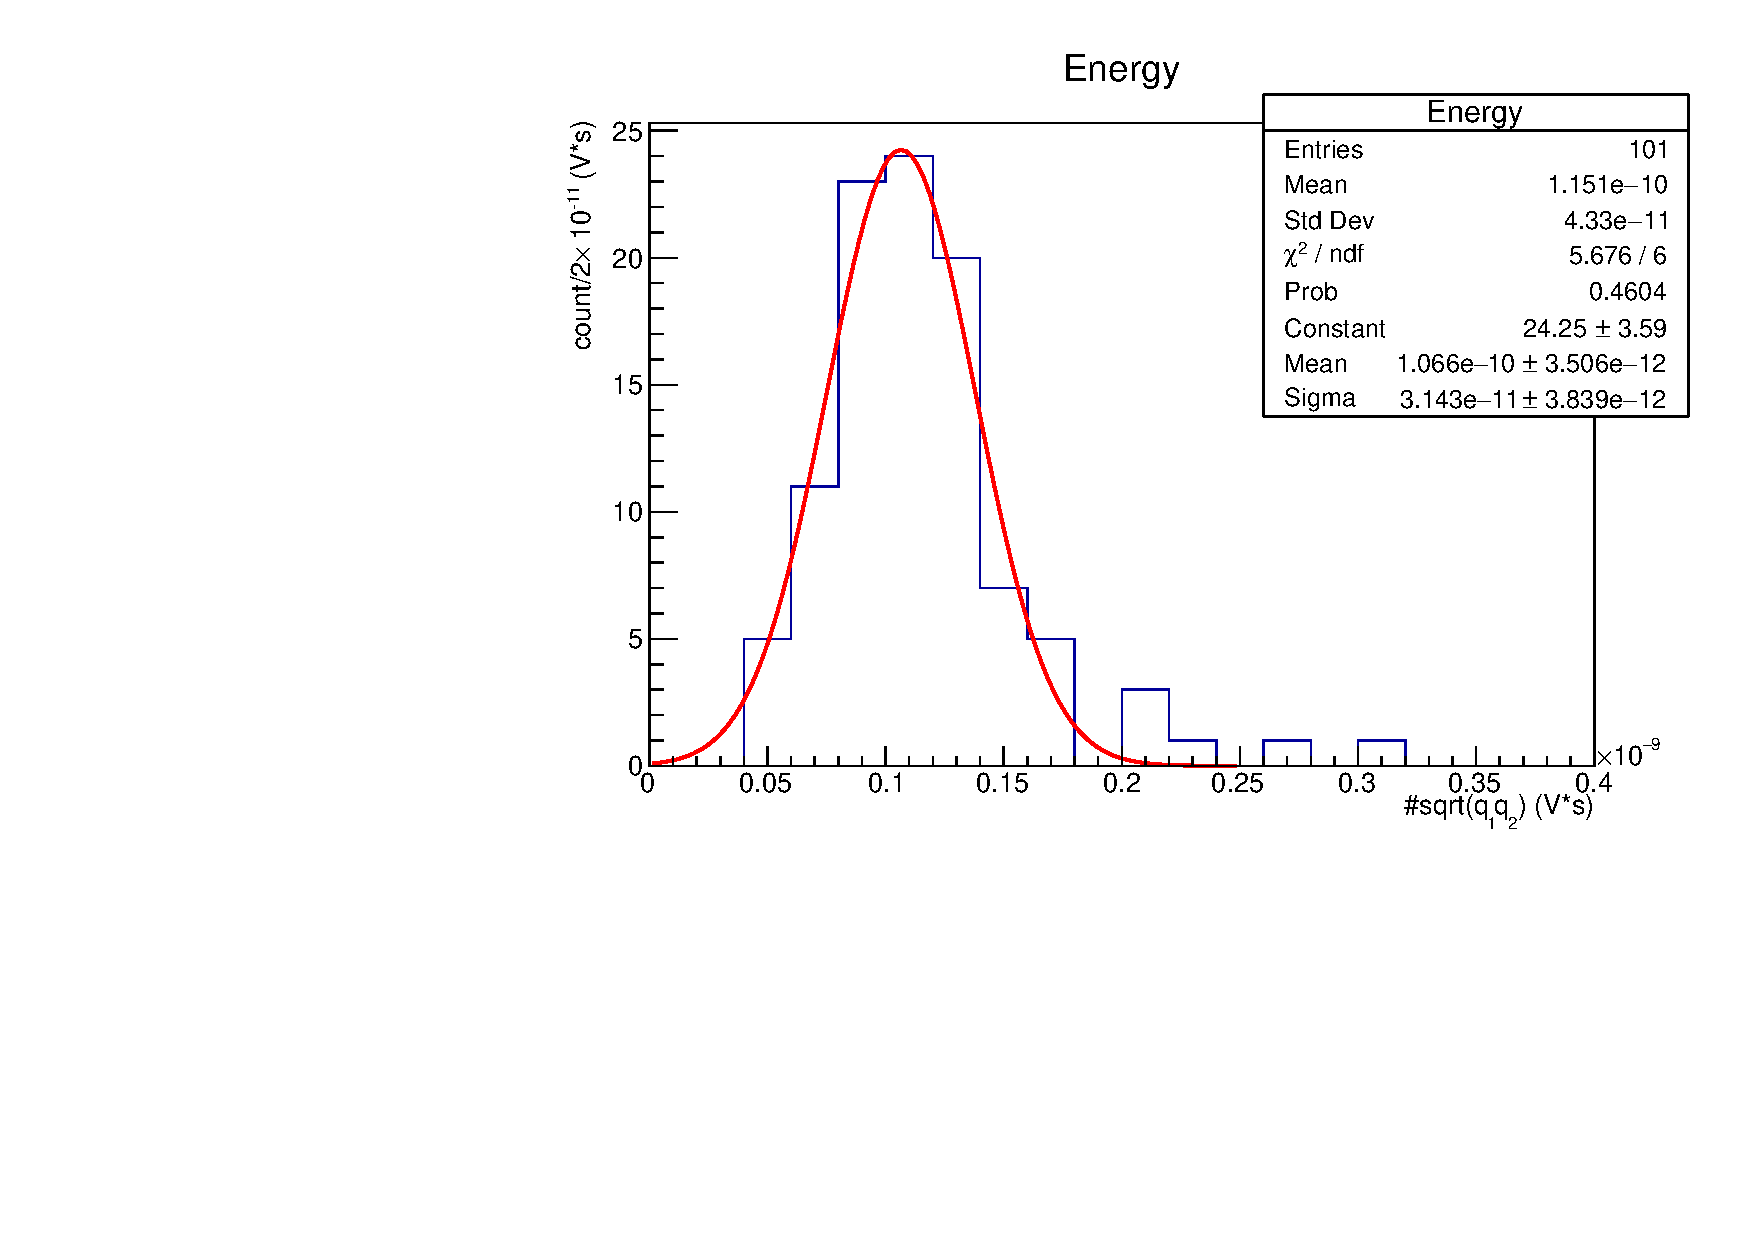
\includegraphics[width=0.5\textwidth]{../../DetectorPerform/ECali/qqdist.pdf}
\caption{能量刻度}
\end{figure}

能量分辨率为:
\begin{equation}
\label{eq:4}
\frac{2.35\sigma}{\mu} = \frac{\num{7.386e-11}}{\num{1.066e-10}} = 69.3\%.
\end{equation}
\end{frame}


\begin{frame}[label={sec:org9740b1e}]{\(\mu\) 寿命}
\begin{columns}
\begin{column}{0.5\columnwidth}
\begin{figure}[htbp]
\centering
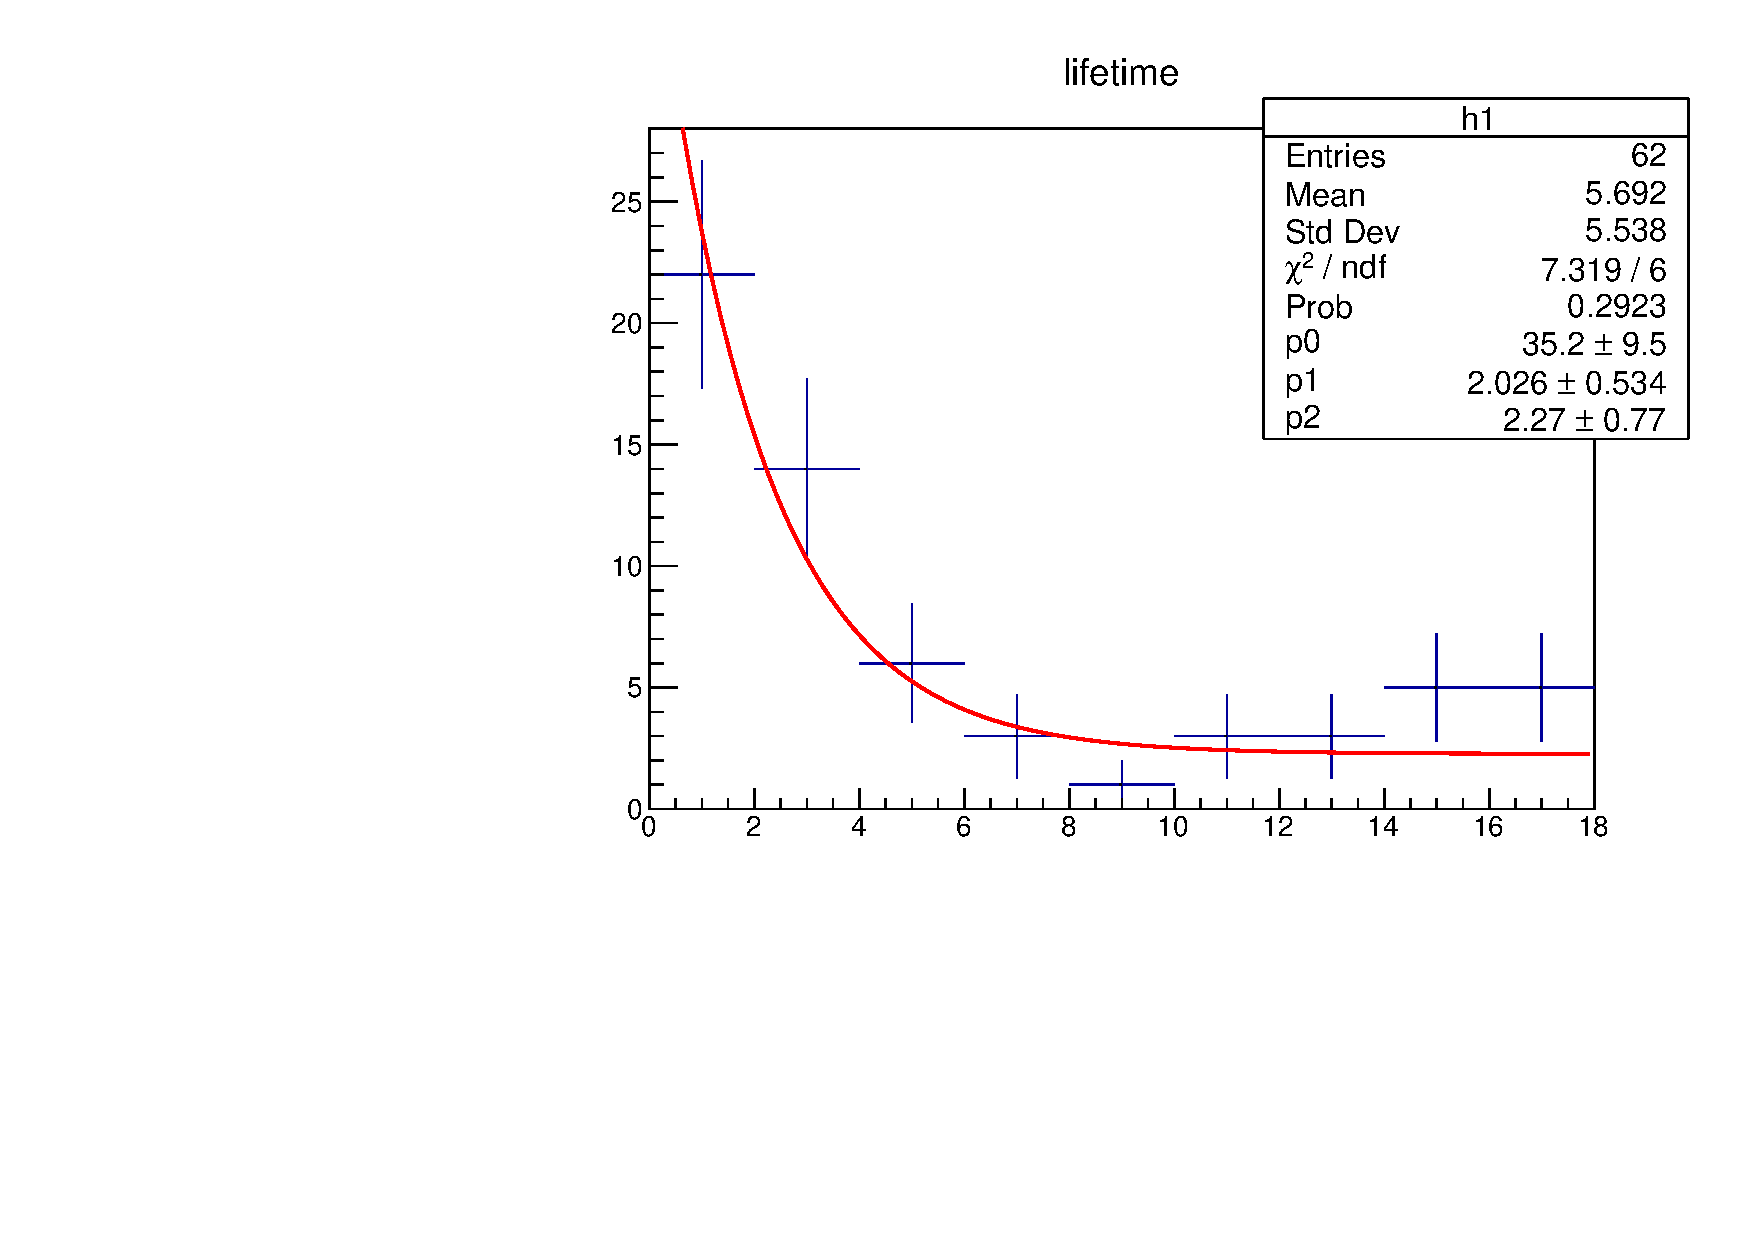
\includegraphics[width=1.0\textwidth]{../../img/lifeTimeHist.pdf}
\caption{\(\mu\) 寿命}
\end{figure}
\end{column}

\begin{column}{0.5\columnwidth}
测得 \(\mu\) 寿命:  
\begin{equation}
\label{eq:5}
\tau = 2.026 \pm \qty{0.534}{\mu s}.
\end{equation}
\end{column}
\end{columns}
\end{frame}

\begin{frame}[label={sec:org90e98c7}]{\(\mu\) 寿命}
同时观察这一部分事例的时间电荷分布, 同样服从线性分布, 且:
\begin{equation}
\label{eq:8}
R^2 = 0.239
\end{equation}
\begin{figure}[htbp]
\centering
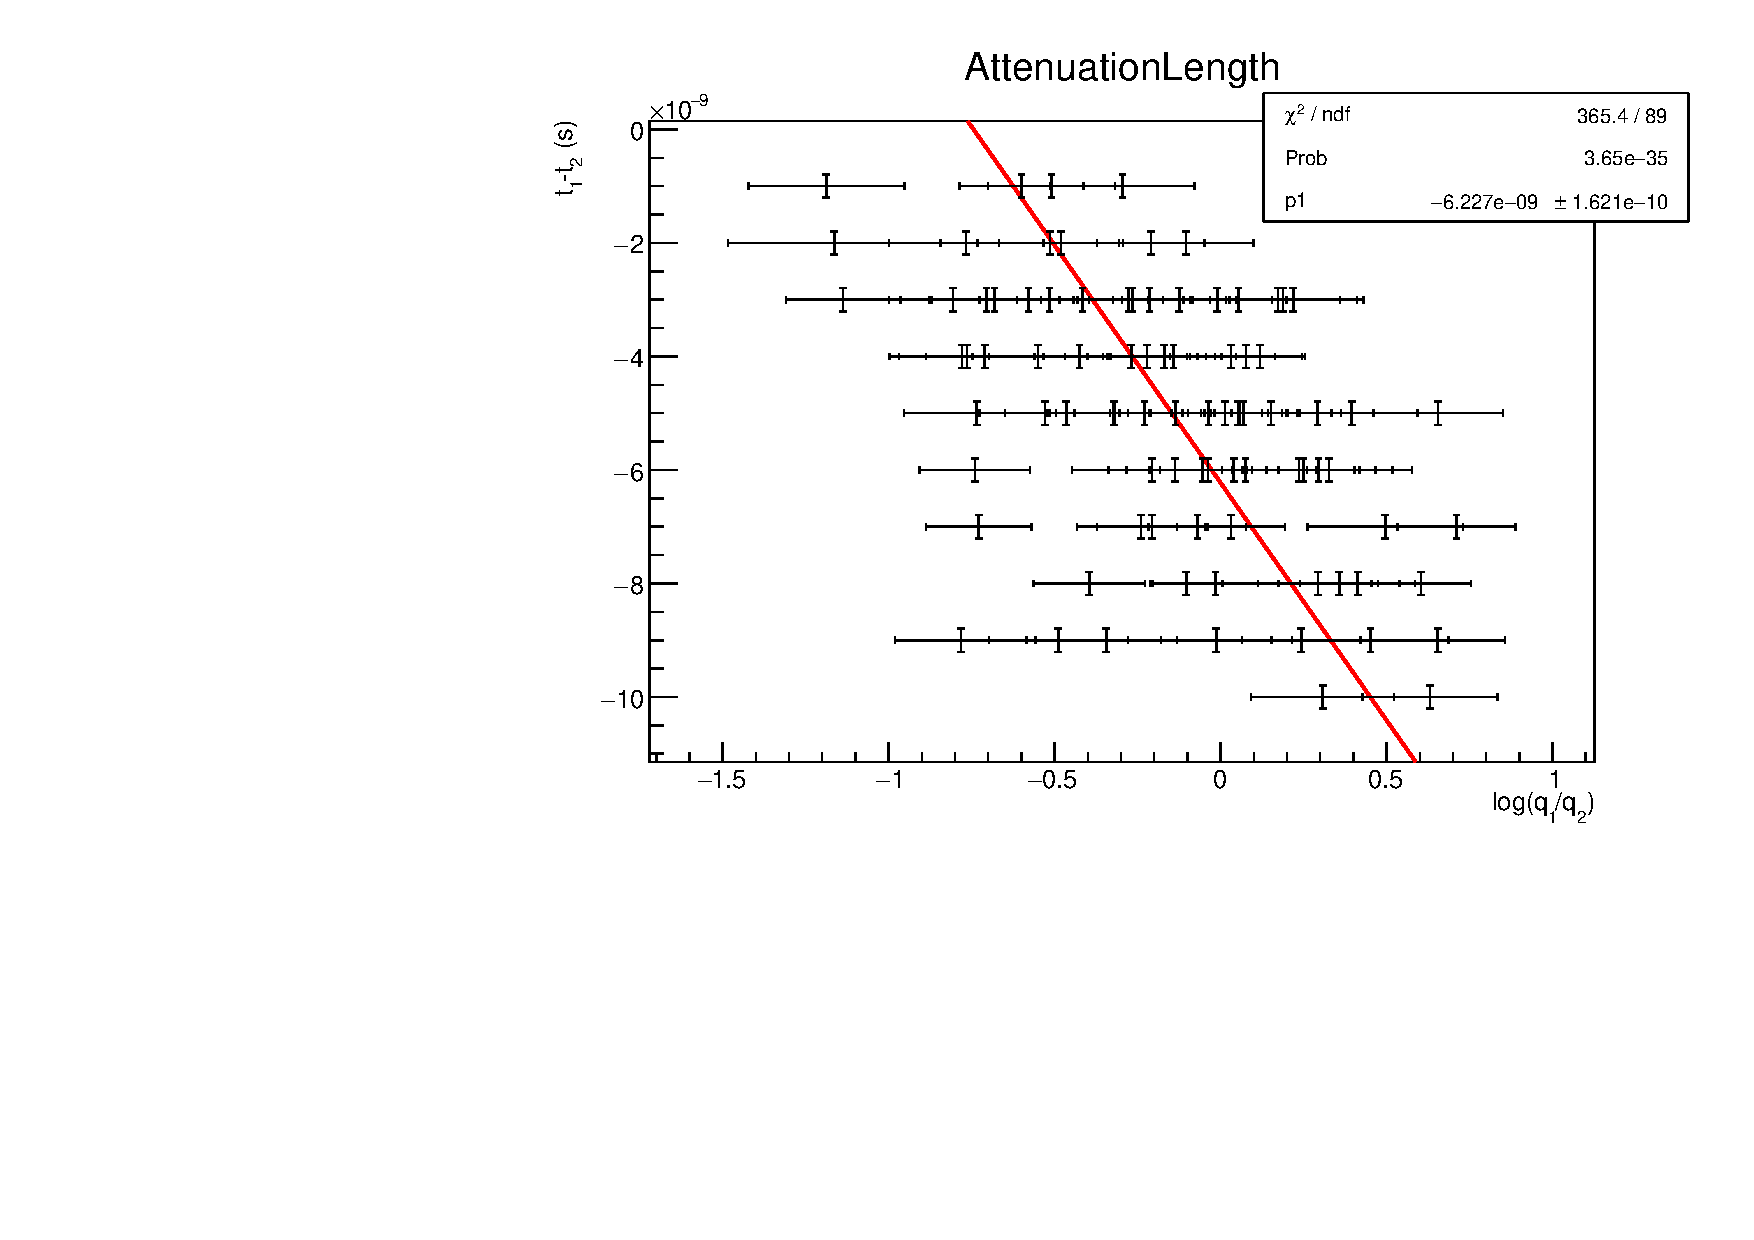
\includegraphics[width=0.6\textwidth]{../../DetectorPerform/AttenuationLength/figs/ReAttenuationLength.pdf}
\caption{时间电荷分布}
\end{figure}
\end{frame}
\end{document}